\chapter{Estudio económico y evaluación económica}

\section{Presupuesto de Costos de producción}

Para la producción durante cada año se incluyen  costos de materiales, mano de obra directa e indirecta, gastos generales de fabricación, entre otros.
Cada categoría de costos se desglosa para mostrar su contribución total al costo de producción por año.

\begin{figure}[H]
    \centering	
    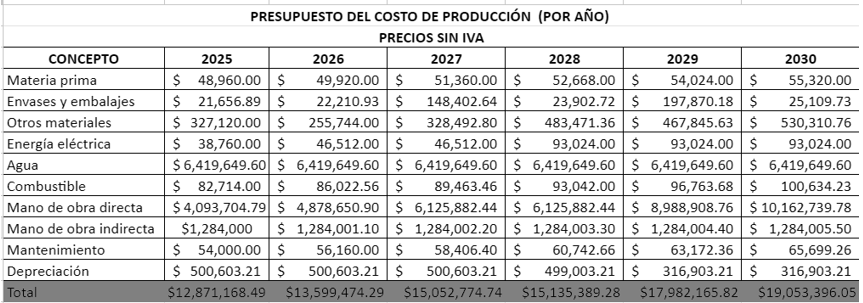
\includegraphics[width=.7\textwidth]{chapters/ELC_1.png} 
    \caption{Presupuesto de costo de producción}
\label{fig:macrolocalizacion}
\end{figure}


\begin{figure}[H]
    \centering	
    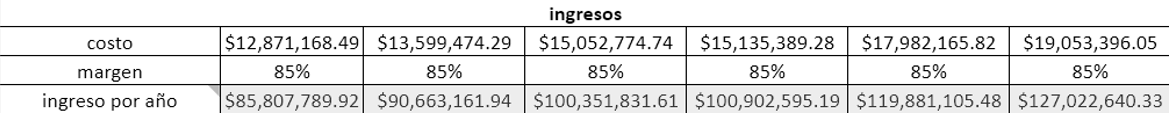
\includegraphics[width=.7\textwidth]{chapters/ELC_2.png} 
    \caption{Ingresos}
\label{fig:macrolocalizacion}
\end{figure}

Esta tabla indica la cantidad total de unidades producidas durante cada período de dos años. Es útil para entender la capacidad de producción utilizada y las fluctuaciones en la demanda a lo largo del tiempo.


\begin{figure}[H]
    \centering	
    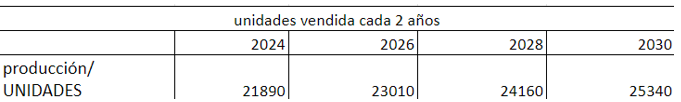
\includegraphics[width=.5\textwidth]{chapters/ELC_3.png} 
    \caption{Unidades de producción}
\label{fig:macrolocalizacion}
\end{figure}

Cada una de estas tablas proporciona información clave para evaluar el desempeño financiero y operativo de la empresa, ayudando a identificar tendencias, eficiencias y áreas de mejora en la gestión de costos, ingresos y producción.

\section{Presupuesto de gastos de administración}


Para realizar el presupuesto se consideraron :Salarios y Honorarios.

Personal Administrativo: Sueldos del personal administrativo responsable de la gestión del proyecto.

Consultores y Asesores: Honorarios para expertos que brinden asesoramiento específico sobre aspectos técnicos, financieros o legales del proyecto.

\begin{figure}[H]
    \centering	
    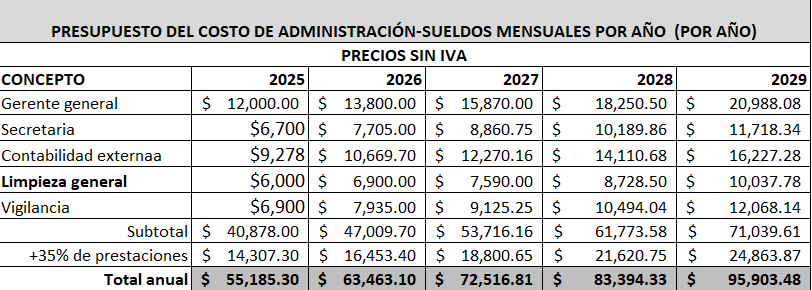
\includegraphics[width=.7\textwidth]{chapters/ELC_4.png} 
    \caption{Presupuestos de administración-sueldos}
\label{fig:macrolocalizacion}
\end{figure}

\begin{figure}[H]
    \centering	
    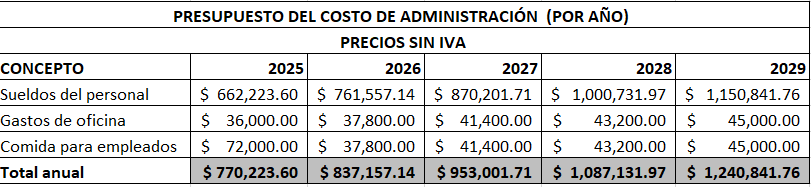
\includegraphics[width=.7\textwidth]{chapters/ELC_5.png} 
    \caption{Presupuestos de administración}
\label{fig:macrolocalizacion}
\end{figure}



\section{Presupuesto de gastos de venta}

Para el presupuesto de gastos para realizar la venta se consideró lo necesario para poder ofrecer el producto y este sea llevado con éxito al cliente, para ello se contempló el gerente de ventas, ingenieros, obreros, choferes, contadores y auxiliares.

\begin{figure}[H]
    \centering	
    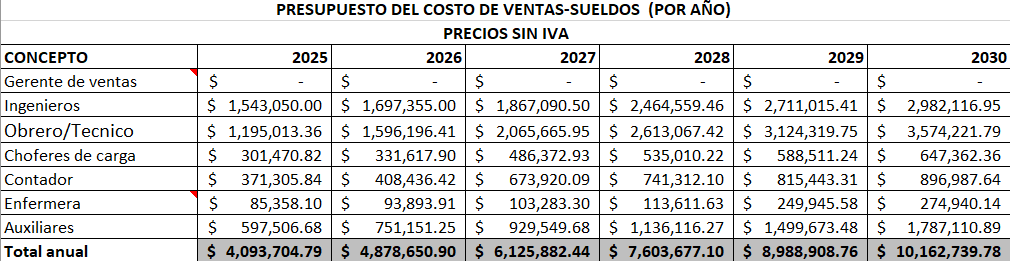
\includegraphics[width=.9\textwidth]{chapters/ELC_6.png} 
    \caption{Presupuestos de ventas-sueldos}
\label{fig:macrolocalizacion}
\end{figure}

\begin{figure}[H]
    \centering	
    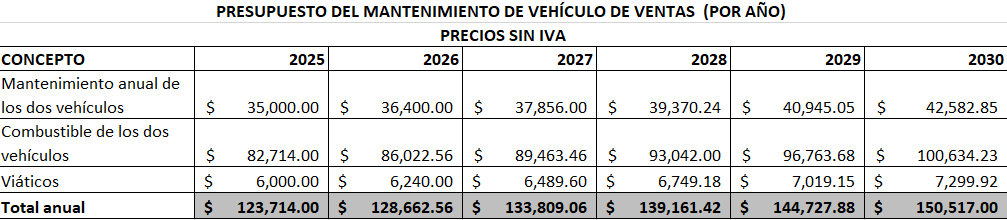
\includegraphics[width=.8\textwidth]{chapters/ELC_7.png} 
    \caption{resupuesto de mantenimiento de vehículo de ventas}
\label{fig:macrolocalizacion}
\end{figure}

\begin{figure}[H]
    \centering	
    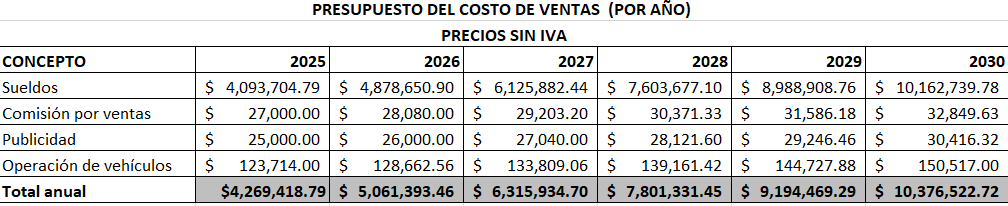
\includegraphics[width=.8\textwidth]{chapters/ELC_8.png} 
    \caption{Presupuestos de costo de ventas}
\label{fig:macrolocalizacion}
\end{figure}


\section{Costo total de operación de la empresa}

\begin{figure}[H]
    \centering	
    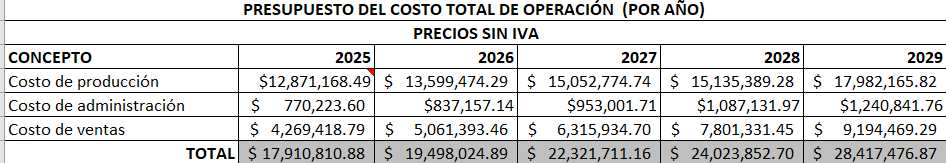
\includegraphics[width=.7\textwidth]{chapters/ELC_9.png} 
    \caption{Costo total de operación}
\label{fig:macrolocalizacion}
\end{figure}




\section{Inversión inicial en activo fijo y diferido}






\subsection{ Inversión fija}

A continuación, se presenta un análisis de inversión fija basándonos en
los documentos y con la investigación de los precios actuales según las
entidades correspondientes al concepto se realizaron los cálculos en los
apartados siguientes.

\subsubsection{Adquisición del terreno }


\hspace{1cm}

\begin{quote}


\textbf{Costo del terreno y gastos por adquisición}

El las siguientes tablas se presentas los debidos costos que se pagaran
para el tramite de la propiedad el cual se realizaran los tramites en
menos de un mes considerando que se tengan los papeles correspondientes
y no se presente algún inconveniente.
\hspace{1cm}


\end{quote}

\begin{longtable}[]{@{}
  >{\raggedright\arraybackslash}p{(\columnwidth - 8\tabcolsep) * \real{0.4331}}
  >{\raggedright\arraybackslash}p{(\columnwidth - 8\tabcolsep) * \real{0.1227}}
  >{\raggedright\arraybackslash}p{(\columnwidth - 8\tabcolsep) * \real{0.1562}}
  >{\raggedright\arraybackslash}p{(\columnwidth - 8\tabcolsep) * \real{0.1337}}
  >{\raggedright\arraybackslash}p{(\columnwidth - 8\tabcolsep) * \real{0.1543}}@{}}
\toprule()
\begin{minipage}[b]{\linewidth}\raggedright
\textbf{CONCEPTO}
\end{minipage} & \begin{minipage}[b]{\linewidth}\raggedright
\textbf{UNIDAD}
\end{minipage} & \begin{minipage}[b]{\linewidth}\raggedright
\textbf{CANTIDAD}
\end{minipage} & \begin{minipage}[b]{\linewidth}\raggedright
\textbf{P.U}
\end{minipage} & \begin{minipage}[b]{\linewidth}\raggedright
\textbf{TOTAL}
\end{minipage} \\
\midrule()
\endhead
Terreno & M2 & 560 & \$1600 & \$896 000 \\
& & & \textbf{Sub total} & \$896 000 \\
\textbf{Escrituración} & & & & \\
Avaluó de inmuebles & \% & 0.13 & \$896 000 & \$1164.8 \\
Adquisición de inmuebles ABI & \% & 2.0 & \$896 000 & \$17920 \\
Certificado de libertad de gravámenes & Tramite & 1.0 & \$100 & \$100 \\
Gastos de papeleo y copias en la notaria & Tramite & 1.0 & \$900 &
\$900 \\
Avisos preventivos y certificados & Tramite & 1.0 & \$500 & \$500 \\
Inscripción al registro publico de la propiedad & \% & 0.075 & \$896 000
& \$672 \\
Honorarios del notario & \% & 1.5 & \$450 000 & \$13440 \\
\multicolumn{3}{@{}>{\raggedright\arraybackslash}p{(\columnwidth - 8\tabcolsep) * \real{0.7120} + 4\tabcolsep}}{%
\multirow{2}{*}{}} & \textbf{Sub total} & \$34696.8 \\
& & & \textbf{TOTAL} & \$930 696.8 \\
\bottomrule()
\end{longtable}

\begin{quote}

Costos y gastos de adquisición

La tabla presentaba anteriormente cubre los costos para la escrituración
dando un total de \$930 696.8 esto es sin contemplar la urbanización,
promediando la realización de este en un mes.

Para el siguiente mes se realizará la urbanización entre los cuales se
incluirán necesariamente los siguientes conceptos.

\hspace{2cm}

\textbf{Costos por permisos y licencias}
\end{quote}

\begin{longtable}[]{@{}
  >{\raggedright\arraybackslash}p{(\columnwidth - 8\tabcolsep) * \real{0.4605}}
  >{\raggedright\arraybackslash}p{(\columnwidth - 8\tabcolsep) * \real{0.1240}}
  >{\raggedright\arraybackslash}p{(\columnwidth - 8\tabcolsep) * \real{0.1579}}
  >{\raggedright\arraybackslash}p{(\columnwidth - 8\tabcolsep) * \real{0.1227}}
  >{\raggedright\arraybackslash}p{(\columnwidth - 8\tabcolsep) * \real{0.1348}}@{}}
\toprule()
\begin{minipage}[b]{\linewidth}\raggedright
\textbf{CONCEPTO}
\end{minipage} & \begin{minipage}[b]{\linewidth}\raggedright
\textbf{UNIDAD}
\end{minipage} & \begin{minipage}[b]{\linewidth}\raggedright
\textbf{CANTIDAD}
\end{minipage} & \begin{minipage}[b]{\linewidth}\raggedright
\textbf{P.U}
\end{minipage} & \begin{minipage}[b]{\linewidth}\raggedright
\textbf{TOTAL}
\end{minipage} \\
\midrule()
\endhead
Lotificación & M2 & 7000 & 2 & \$14 000 \\
Costo por cada lote resultante (en este caso 2) & Lote & 2 & 500 & \$1
000 \\
Aprobación del proyecto & M2 & \$896 000 & 0.6 & \$5376 \\
Uso del suelo & M2 & \$896 000 & 1.6 & \$14336 \\
Licencia de construcción de la barda & M2 & \$896 000 & 7.5 & \$36000 \\
\multicolumn{4}{@{}>{\raggedright\arraybackslash}p{(\columnwidth - 8\tabcolsep) * \real{0.8652} + 6\tabcolsep}}{%
} & \$70712 \\
\bottomrule()
\end{longtable}

\hspace{1cm}


\begin{quote}
Costos por permisos y licencias

\textbf{Costos de urbanización por partida}
\end{quote}

\begin{longtable}[]{@{}
  >{\raggedright\arraybackslash}p{(\columnwidth - 4\tabcolsep) * \real{0.3375}}
  >{\raggedright\arraybackslash}p{(\columnwidth - 4\tabcolsep) * \real{0.3269}}
  >{\raggedright\arraybackslash}p{(\columnwidth - 4\tabcolsep) * \real{0.3356}}@{}}
\toprule()
\begin{minipage}[b]{\linewidth}\raggedright
Partida
\end{minipage} & \begin{minipage}[b]{\linewidth}\raggedright
\%
\end{minipage} & \begin{minipage}[b]{\linewidth}\raggedright
costo/M2
\end{minipage} \\
\midrule()
\endhead
Agua potable & 11.0\% & \$150 250 \\
Condiciones generales & 9.5\% & \$250 251 \\
Drenaje pluvial & 2.3\% & \$75 256 \\
Electrificado y alumbrado & 5.2\% & \$132 025 \\
Terracerías & 6.2\% & \$145 256 \\
Pavimentos y banquetas & 4.1\% & \$128 185 \\
Totales & & \$881 223 \\
\bottomrule()
\end{longtable}

\begin{quote}
Costos de urbanización por m2

Los apartados anteriores forman partes de la inversión para la
adquisición del terreno y puesta en marcha para el inicio de la
construcción de la planta a lo cual el costo total es englobado en la
siguiente tabla.

\hspace{1cm}

\newpage

\textbf{Costo total del terreno más adquisición}
\end{quote}

\begin{longtable}[]{@{}
  >{\raggedright\arraybackslash}p{(\columnwidth - 4\tabcolsep) * \real{0.3377}}
  >{\raggedright\arraybackslash}p{(\columnwidth - 4\tabcolsep) * \real{0.3305}}
  >{\raggedright\arraybackslash}p{(\columnwidth - 4\tabcolsep) * \real{0.3319}}@{}}
\toprule()
\begin{minipage}[b]{\linewidth}\raggedright
CONCEPTO
\end{minipage} & \begin{minipage}[b]{\linewidth}\raggedright
\%
\end{minipage} & \begin{minipage}[b]{\linewidth}\raggedright
TOTAL
\end{minipage} \\
\midrule()
\endhead
Adquisición del terreno & & \$896 000 \\
Escrituras y tramites & & \$34 696.8 \\
Urbanización y lotificación & & \$881 223 \\
Construcción de barda & & \$150 254 \\
Proyecto ejecutivo & & \$120 581 \\
Permisos y licencias & & \$72 252 \\
\textbf{Total} & \textbf{100\%} & \textbf{\$2 155 006.8} \\
\bottomrule()
\end{longtable}

\begin{quote}
Costos totales de adquisición del terreno

El costo total para iniciar con la construcción de la planta será de
\textbf{\$2 155 006.8} teniendo el capital para la inversión cubriendo
en su totalidad el pago sin requerir por esta vez la solicitud de un
préstamo bancario o externo, disminuyendo el precio para poder invertir
en los demás aspectos.

4.2. Obra civil.
\end{quote}

En este apartado se realizan los presupuestos poyados por la
documentación generado por arquitectos y constructores sobre el cual se
genera un documento con los requerimientos específicos, ¡normativas,
materiales, presupuestos usos del espacio y tecnología a utilizar.

\begin{longtable}[]{@{}
  >{\raggedright\arraybackslash}p{(\columnwidth - 4\tabcolsep) * \real{0.2311}}
  >{\raggedright\arraybackslash}p{(\columnwidth - 4\tabcolsep) * \real{0.1361}}
  >{\raggedright\arraybackslash}p{(\columnwidth - 4\tabcolsep) * \real{0.6327}}@{}}
\toprule()
\multicolumn{3}{@{}>{\raggedright\arraybackslash}p{(\columnwidth - 4\tabcolsep) * \real{1.0000} + 4\tabcolsep}@{}}{%
\begin{minipage}[b]{\linewidth}\raggedright
\textbf{Proyecto de construcción}
\end{minipage}} \\
\midrule()
\endhead
\multicolumn{3}{@{}>{\raggedright\arraybackslash}p{(\columnwidth - 4\tabcolsep) * \real{1.0000} + 4\tabcolsep}@{}}{%
\textbf{Proyecto de planta}} \\
\multicolumn{3}{@{}>{\raggedright\arraybackslash}p{(\columnwidth - 4\tabcolsep) * \real{1.0000} + 4\tabcolsep}@{}}{%
\textbf{Área total del lote} 560 m\textsuperscript{2} \textbf{Área de
planta baja} 250 m\textsuperscript{2}

\textbf{Área de construcción} 360 m\textsuperscript{2} \textbf{Áreas de
planta alta} 110 m\textsuperscript{2}} \\
\multicolumn{3}{@{}>{\raggedright\arraybackslash}p{(\columnwidth - 4\tabcolsep) * \real{1.0000} + 4\tabcolsep}@{}}{%
\textbf{Primer nivel-Distribución}} \\
Comedor & 18.6m\textsuperscript{2} &
\multirow{13}{*}{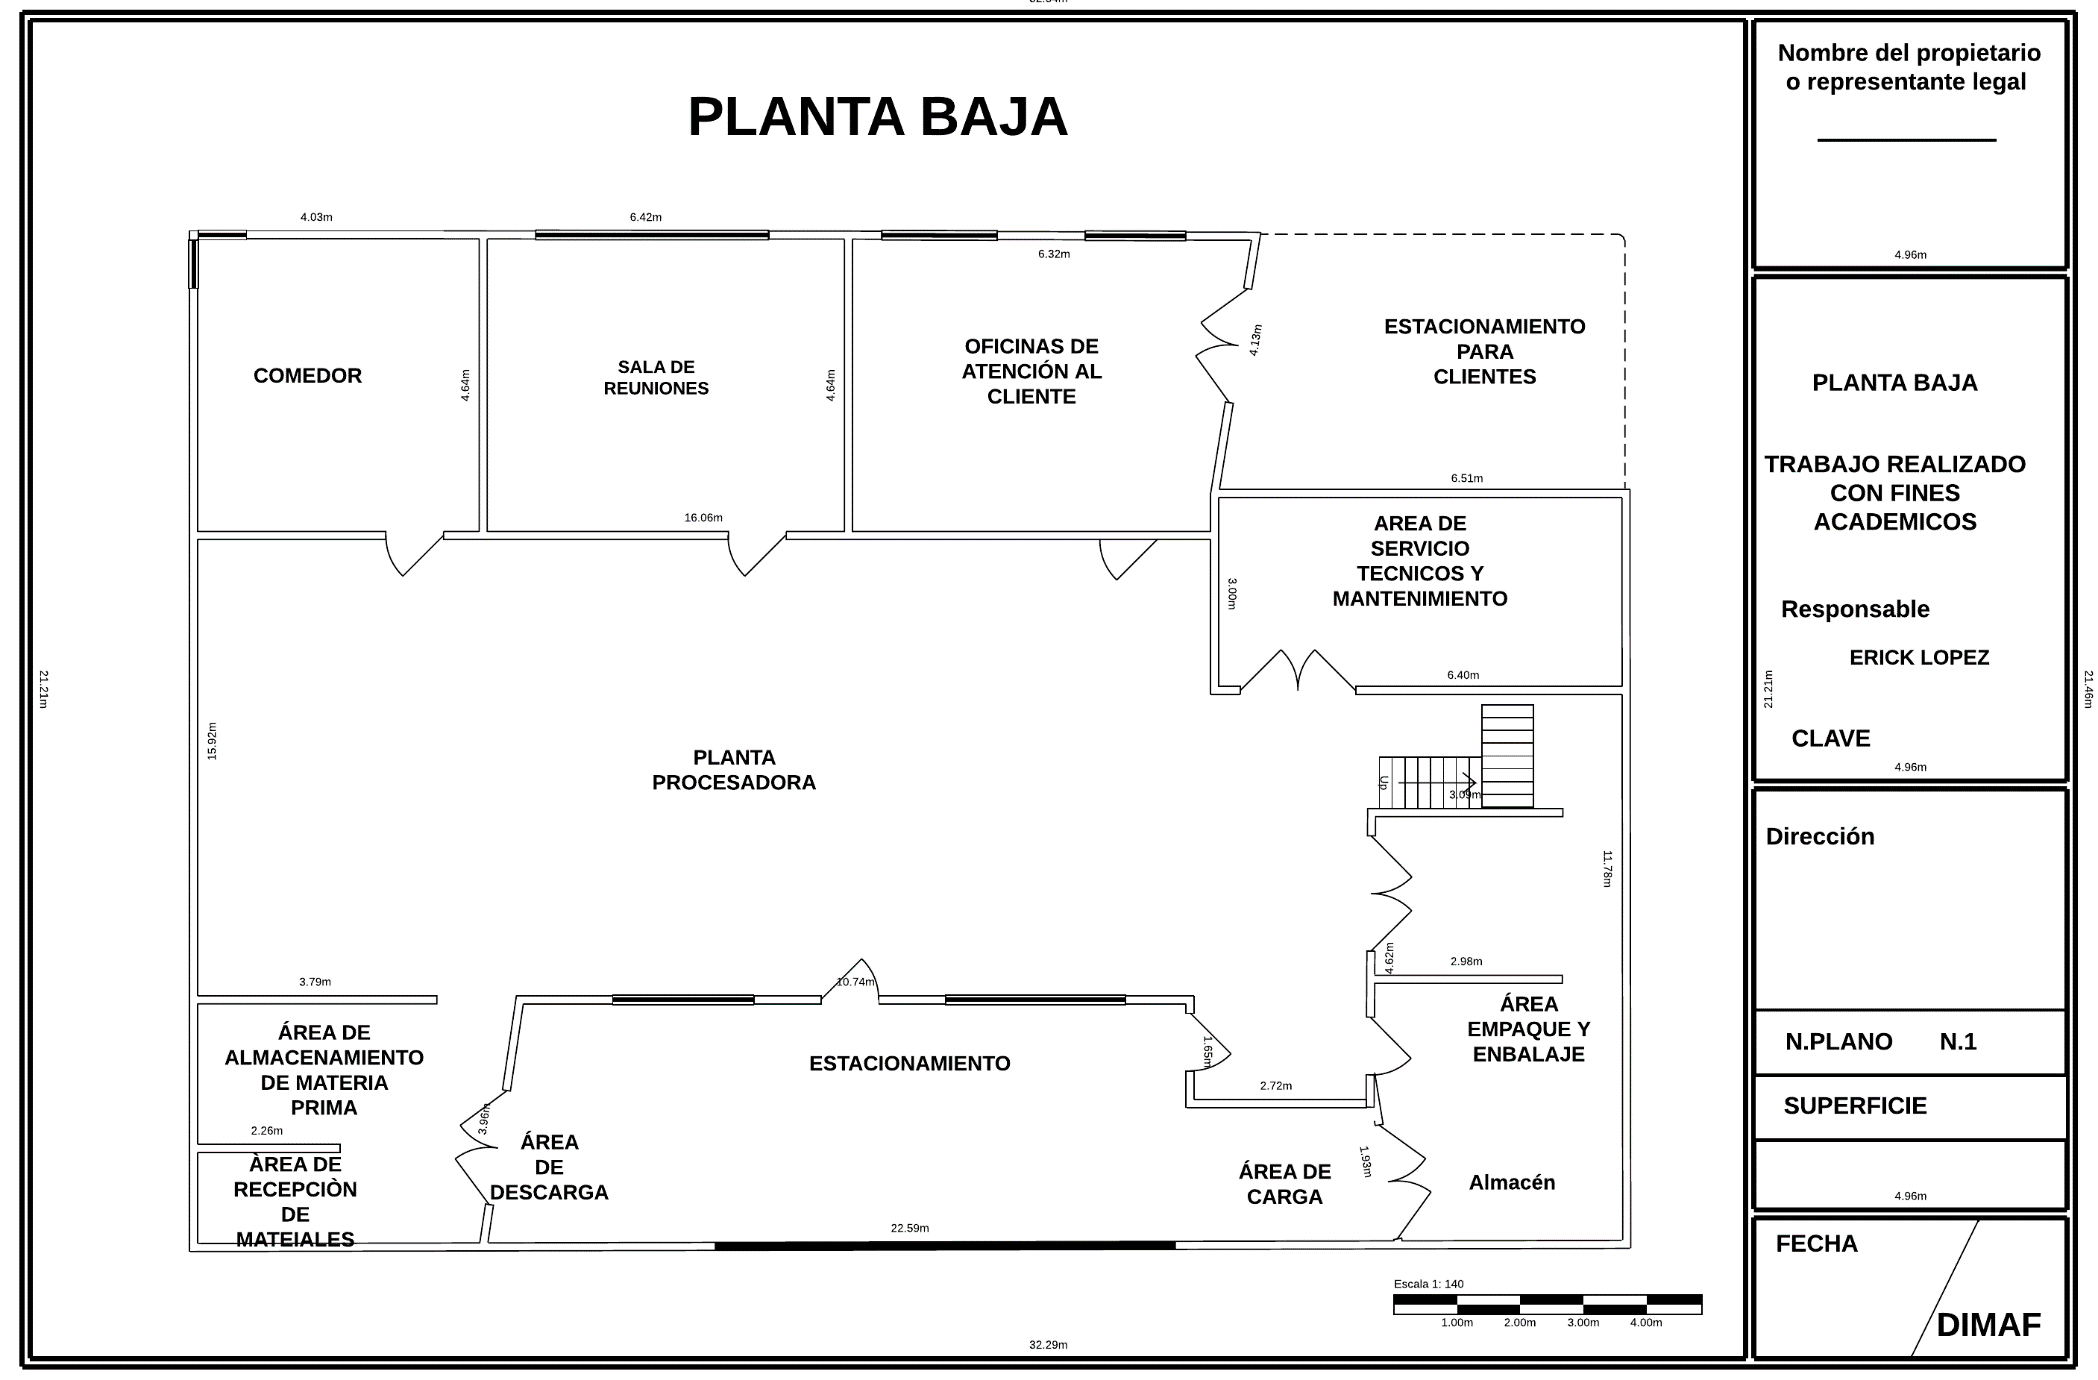
\includegraphics[width=4.22565in,height=3.04844in]{chapters/image1_.png}

} \\

Oficina de atención al cliente & 29.78m\textsuperscript{2} \\
Estacionamiento de clientes & 26.88m\textsuperscript{2} \\
Área de servicio técnico y mantenimiento & 19.2m\textsuperscript{2} \\
Área de empaque y embalaje & 6m\textsuperscript{2} \\
Almacén & 9m\textsuperscript{2} \\
Área de carga & 6m\textsuperscript{2} \\
Área de descarga & 10m\textsuperscript{2} \\
Estacionamiento para la empresa & 30m\textsuperscript{2} \\
Área de recepción de materiales & 6m\textsuperscript{2} \\
Área de almacenamiento de materias prima & 12m\textsuperscript{2} \\
Sala de reuniones & 28m\textsuperscript{2} \\
Planta procesadora & 370m\textsuperscript{2} \\
\multicolumn{3}{@{}>{\raggedright\arraybackslash}p{(\columnwidth - 4\tabcolsep) * \real{1.0000} + 4\tabcolsep}@{}}{%


\textbf{Segundo nivel-Distribución}} \\
Oficina 1 & 20m\textsuperscript{2} &
\multirow{4}{*}
{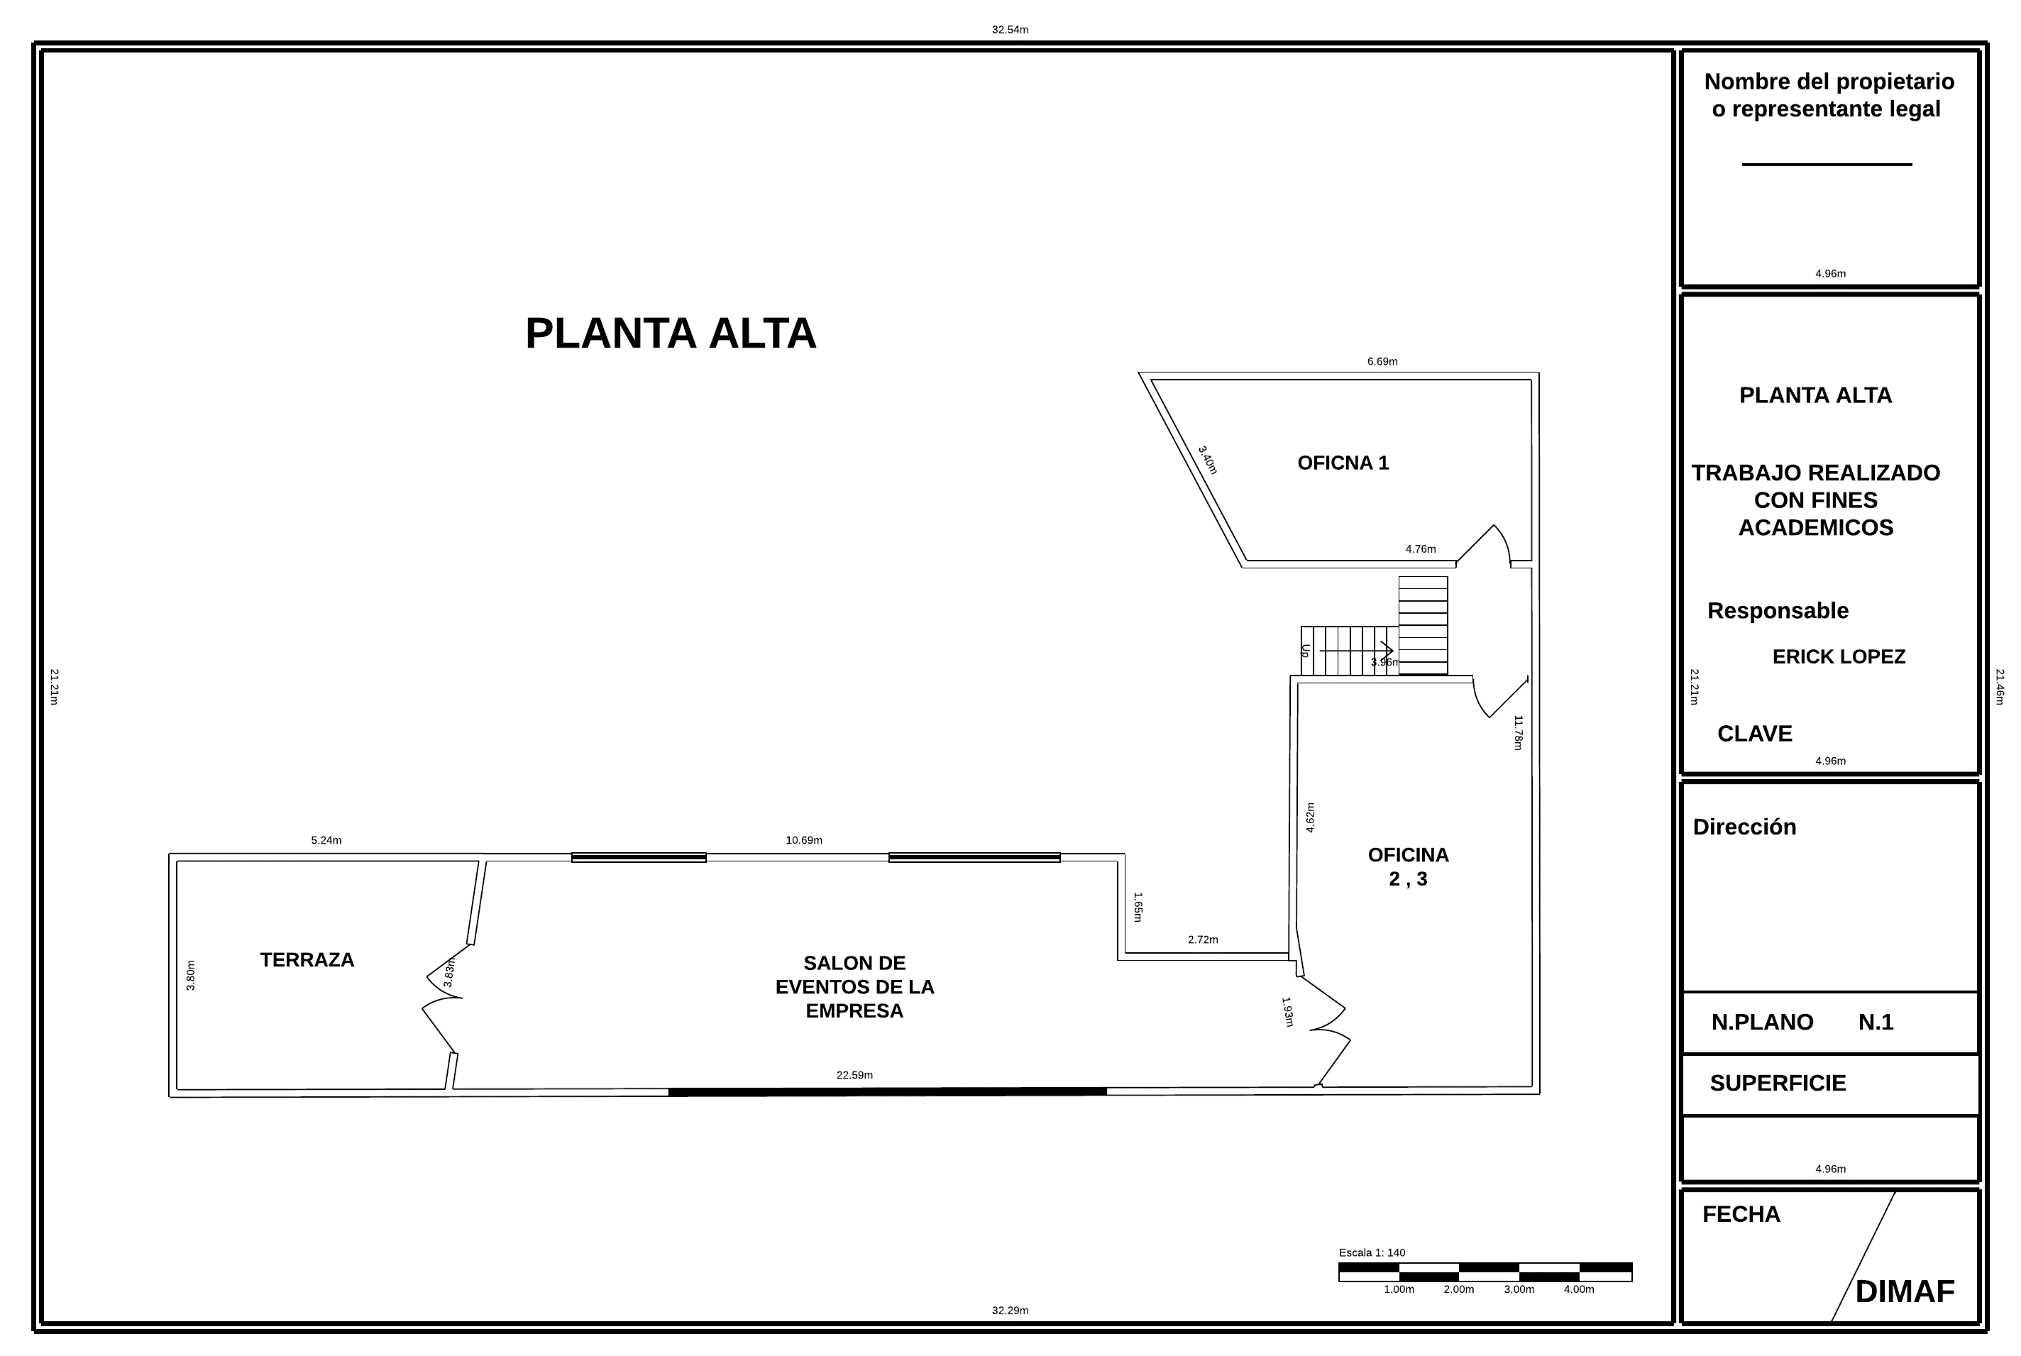
\includegraphics[width=3.95825in,height=2.13528in]{chapters/image2_.png}} \\
\hspace{2cm}
Oficina 2,3 & 39.2m\textsuperscript{2} \\
Salón de eventos & 42.2m\textsuperscript{2} \\
Terraza & 20.1m\textsuperscript{2} \\
\hspace{4cm}
\bottomrule()
\end{longtable}


\hspace{2cm}

Características geométricas de la distribución de los departamentos de
la empresa. Elaboración propia.







\subsubsection{Obra civil}




\subsection{Obra civil}

\begin{figure}[H]
    \centering	
    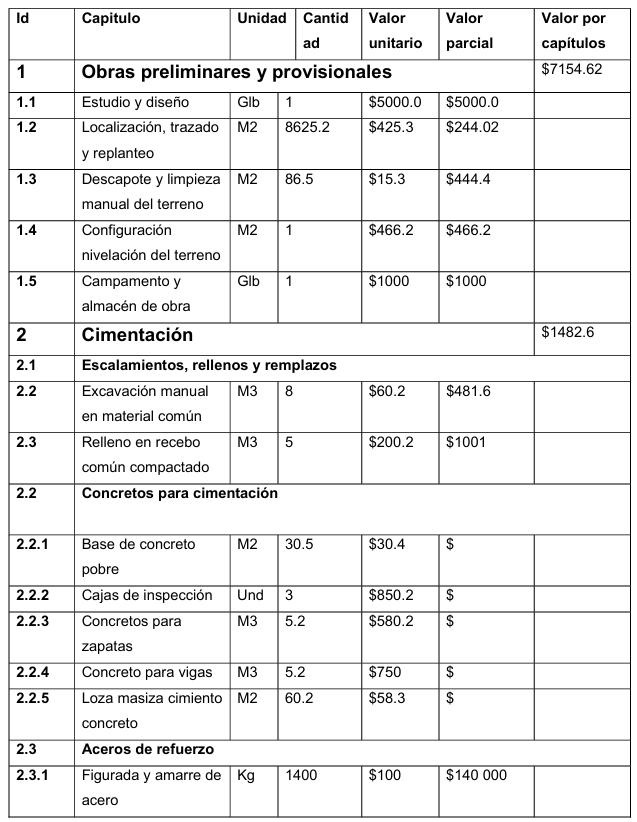
\includegraphics[width=1.0\textwidth]{chapters/ELC1.png} 
    \caption{Presupuesto de obra civil parte 1}
\label{fig:croquis190125}
\end{figure}

\begin{figure}[H]
    \centering	
    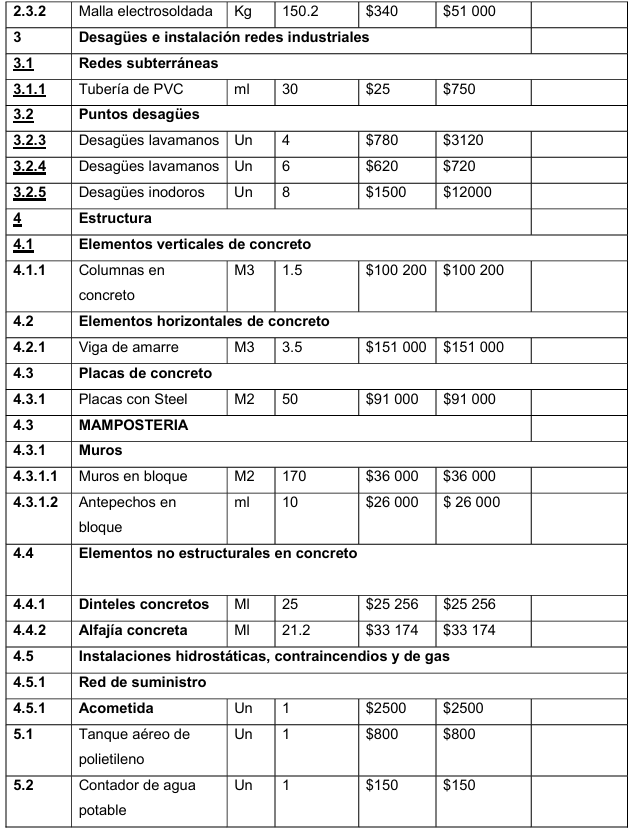
\includegraphics[width=1.0\textwidth]{chapters/ELC2.png} 
    \caption{Presupuesto de obra civil parte 2}
\label{fig:croquis190125}
\end{figure}

\begin{figure}[H]
    \centering	
    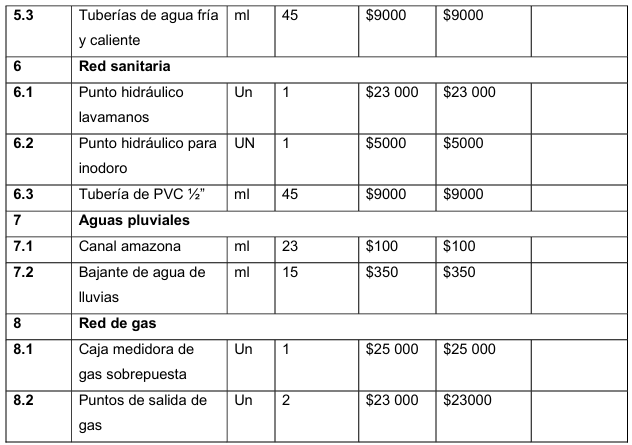
\includegraphics[width=1.0\textwidth]{chapters/ELC3.png} 
    \caption{Presupuesto de obra civil parte 3}
\label{fig:croquis190125}
\end{figure}


Para la construcción de la obra se tiene que invertir un aproximado de 3 251 125 pesos para poder tener la edificación y desde esta poder operar de manera adecuada y cómoda. 

%-------------------





\subsubsection{Adquisición de la tecnología de producción}

\begin{figure}[H]
    \centering	
    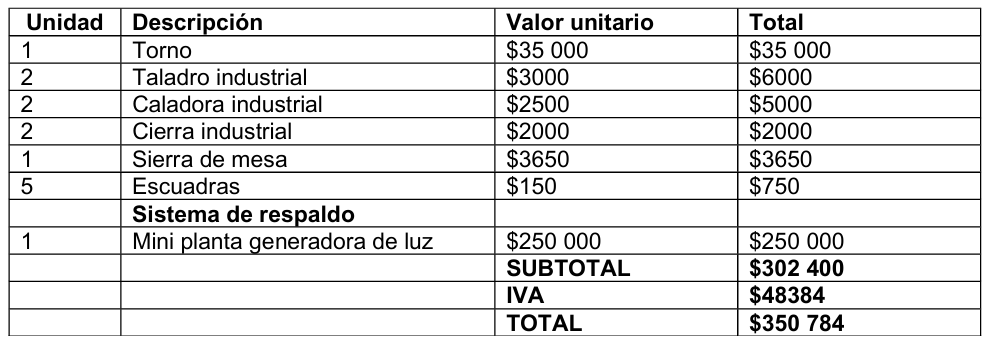
\includegraphics[width=1.1\textwidth]{chapters/ELC4.png} 
    \caption{Presupuesto de adquisición de tecnología }
\label{fig:croquis190125}
\end{figure}



\subsubsection{Adquisición de mobiliario y oficina}

\begin{figure}[H]
    \centering	
    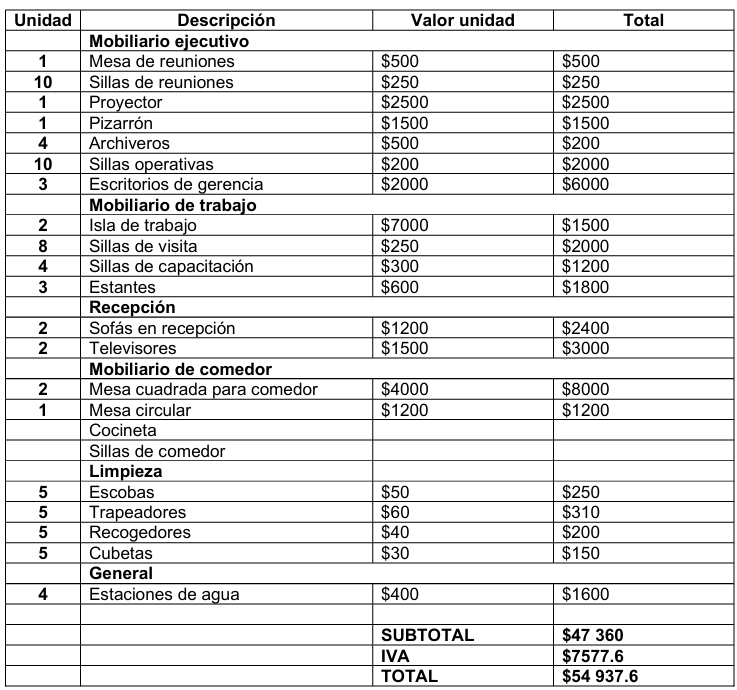
\includegraphics[width=1.1\textwidth]{chapters/ELC5.png} 
    \caption{Presupuesto de adquisición de mobiliario y oficina }
\label{fig:croquis190125}
\end{figure}

En la adquisición de mobiliario de oficina se tomo encuentra al mobiliario tanto de los ejecutivos, de los trabajadores, al que se colocaría en recepción, el comedor , la limpieza y generales ya que en cada uno de ellos se utilizan diferentes equipos de uso indispensable. 


\subsubsection{Adquisición del equipo de computo}

\begin{figure}[H]
    \centering	
    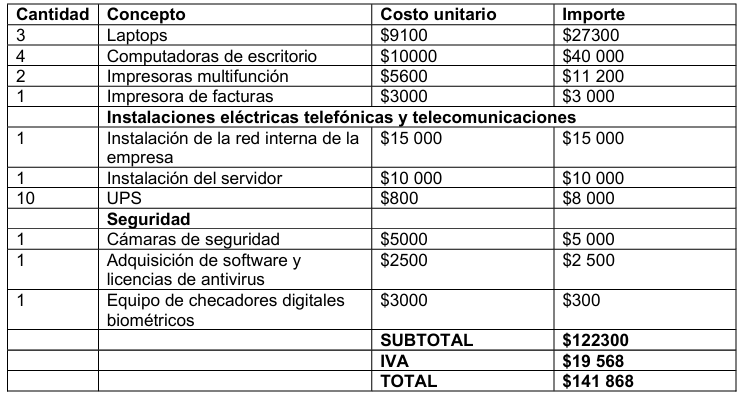
\includegraphics[width=1.1\textwidth]{chapters/ELC6.png} 
    \caption{Presupuesto de adquisición de mobiliario y oficina }
\label{fig:croquis190125}
\end{figure}






\subsection{Inversión diferida}
La inversión diferida se refiere a los gastos que una empresa realiza para obtener beneficios en el futuro, pero que no se consideran como activos fijos. Estos gastos no están destinados a adquirir activos físicos, sino que se utilizan para mejorar o mantener los activos existentes de una empresa.

Incluyen gastos en investigación y desarrollo, capacitación de empleados, publicidad, promoción y mejoras en la calidad de productos o servicios. Estos gastos son necesarios para mantener la competitividad de una empresa en el mercado y generar mayores ingresos en el futuro.

En los primeros momentos de producción no se espera invertir montos considerables en aspectos que no sean completamente necesarios para la producción, sin embargo se proponen las siguientes inversiones diferidas.

\begin{table}[h]
    \centering
    \caption{Inversión diferida bimestral}
    \begin{tabular}{p{5cm} || p{2cm} || p{3cm} || p{3cm}}
        \toprule
        \textbf{Concepto de Inversión Diferida} & \textbf{Precio mensual} & \textbf{Precio bimestral} & \textbf{Total bimestral}\\
        \midrule
        Capacitación de empleados & \$5,000 &\$10,000 &\\
        Mantenimiento de equipo & \$1,500 & \$3,000&\\
        Internet & \$1,000 & \$2,000&\\
        Luz & \$4,000 & \$8,000&\\
        Agua & \$600 & \$1,200 &\\
        Transporte & \$1,000 & \$2,000 &\\
        Publicidad & \$750 & \$1,500 &\\
        \hline
        IVA(16\%) & \$2,216 & \$4,432 & \$32,132\\
        \bottomrule
    \end{tabular}
\end{table}




\section{Depreciación y amortización}

\begin{figure}[H]
    \centering	
    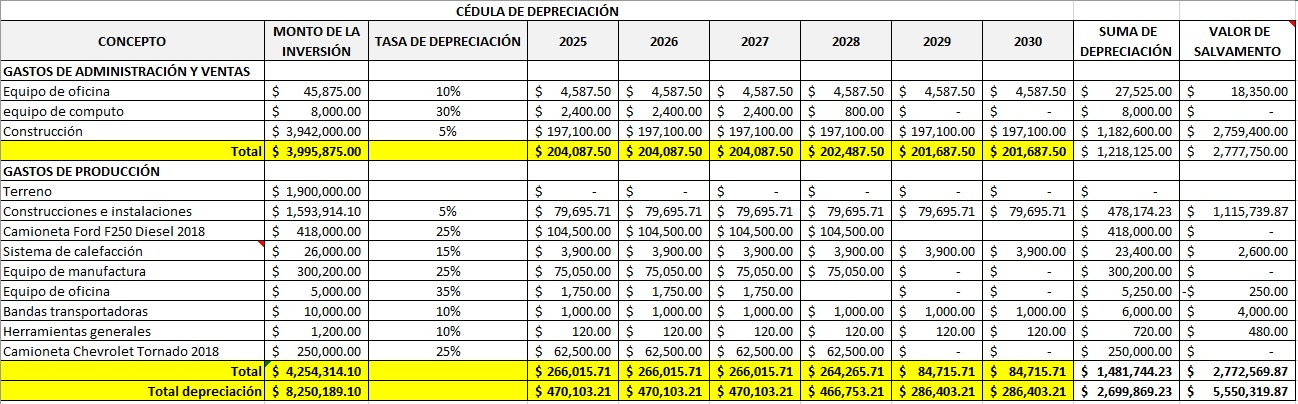
\includegraphics[width=1.1\textwidth]{chapters/ELC_10.png} 
    \caption{Célula de depreciación}
\label{fig:croquis190125}
\end{figure}



\section{Financiamiento de la inversión}

De los \$4 217 671.5 que se requieren de inversion fija y diferida, se pretende solicitar un prestamo por \$2 millones, el cual se liquidara en seis anualidades iguales, pagando la primera anualidad al final del primer año, por el cual se cobrará un interés de 32\% anual. Esta tasa de interés ya contiene a la inflación pronosticada. La anualidad que se pagará se calcula como:

La deuda equivalente a una aportación porcentual de capital de 47.149\%, por lo que la empresa deberá aportar el 52.58\% total sin incluir capital de trabajo. 

\begin{figure}[H]
    \centering	
    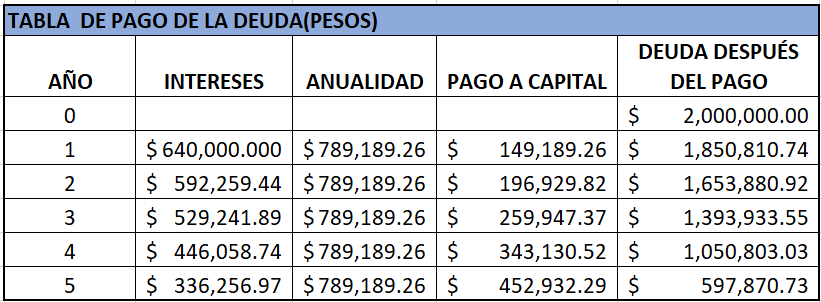
\includegraphics[width=0.9\textwidth]{chapters/ELC_11.png} 
    \caption{Tabla de pago de la deuda}
\label{fig:croquis190125}
\end{figure}


\section{Determinación del capital de trabajo Pasivo circulante}

\begin{table}[htbp]
    \centering
    \begin{tabular}{|l|c|c|c|}
        \hline
        \textbf{Concepto} & \textbf{Costo} & \textbf{IVA} & \textbf{Importe} \\
        \hline
        COSTO DE PRODUCCIÓN & & & \\
        \hline
        Materias primas & \$1000 & \$160 & \$1160 \\
        Materias primas secundarias y materiales indirectos & \$800 & \$128 & \$928 \\
        Sueldos y salarios & \$2500 & \$0 & \$2500 \\
        Gastos indirectos & \$1500 & \$0 & \$1500 \\
        \hline
        SUBTOTAL & & & \$6088 \\
        \hline
        GASTOS DE ADMINISTRACIÓN & & & \\
        \hline
        Sueldos y salarios & \$1000 & \$0 & \$1000 \\
        Gastos indirectos & \$800 & \$0 & \$800 \\
        \hline
        SUBTOTAL & & & \$1800 \\
        \hline
        GASTOS DE VENTA & & & \\
        \hline
        Sueldos y salarios & \$500 & \$0 & \$500 \\
        Gastos indirectos & \$300 & \$0 & \$300 \\
        \hline
        SUBTOTAL & & & \$800 \\
        \hline
        TOTAL & & & \$8688 \\
        \hline
    \end{tabular}
    \caption{Estimación del Capital de Trabajo}
    \label{tab:estimacion_capital_trabajo}
\end{table}

La tabla proporciona una estimación del capital de trabajo necesario para llevar a cabo el proyecto. Se divide en tres secciones principales: costo de producción, gastos de administración y gastos de venta.

En la sección de costo de producción, se detallan los diferentes elementos necesarios para la producción del sistema de control de planta, como materias primas, materiales indirectos y sueldos y salarios asociados con la producción. Además, se incluyen los gastos indirectos que pueden surgir durante este proceso. El subtotal muestra el total de estos costos de producción.

En la sección de gastos de administración, se enumeran los costos asociados con la gestión y administración del proyecto, incluidos los sueldos y salarios del personal administrativo y los gastos indirectos asociados con estas actividades. Nuevamente, se proporciona un subtotal para esta sección.

Finalmente, en la sección de gastos de venta, se presentan los costos relacionados con la promoción y comercialización del producto, como sueldos y salarios del personal de ventas y otros gastos indirectos relacionados con estas actividades. Se calcula un subtotal para esta sección.

El total general muestra la suma de todos los subtotales, proporcionando una estimación del capital de trabajo total necesario para llevar a cabo el proyecto. Esta tabla es útil para tener una idea general de los recursos financieros requeridos y planificar adecuadamente el presupuesto para el proyecto.


\section{Determinación del punto de equilibrio}

El punto de equilibrio es el nivel de producción en el que los ingresos por ventas son exactamente iguales a la suma de los costos fijos y los variables.

Ingresos= costo total

P × Q = CF + CV

Con base en el presupuesto de ingresos y de los costos de producción, administración y ventas, se clasifican los costos como fijos y variables, con la finalidad de determinar cuál es el nivel de producción donde los costos totales se igualan a los ingresos.


\begin{figure}[H]
    \centering	
    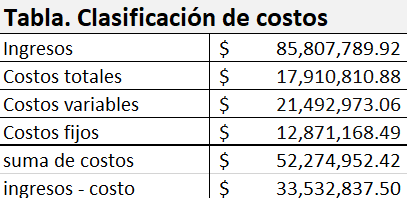
\includegraphics[width=0.6\textwidth]{chapters/ELC_PUNTO2.png} 
    \caption{Clasificación de costos}
\label{fig:croquis190125}
\end{figure}

\begin{figure}[H]
    \centering	
    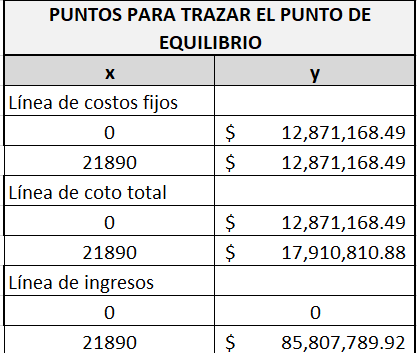
\includegraphics[width=0.6\textwidth]{chapters/ELC_PUNTO3.png} 
    \caption{Puntos para trazar el punto de equilibrio}
\label{fig:croquis190125}
\end{figure}


\begin{figure}[H]
    \centering	
    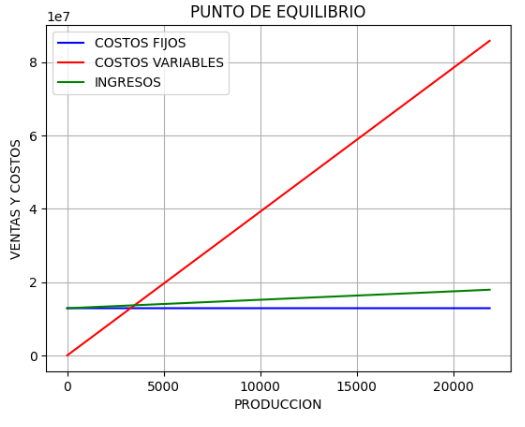
\includegraphics[width=0.9\textwidth]{chapters/ELC_PUNTO.png} 
    \caption{punto de equilibrio}
\label{fig:croquis190125}
\end{figure}



\section{Balance general inicial}

El balance general o balance de situación de una empresa es un documento contable financiero que refleja la situación económica y patrimonial de la misma en una fecha determinada, permite conocer la situación financiera y patrimonial de una compañía en un momento concreto, pues en él se detallan sus activos, sus pasivos y su capital.

La igualdad fundamental del balance:

	\textbf{	Activo = Pasivo + Capital }
  
\textbf{Activo}, representa cualquier pertenencia material o inmaterial de la empresa. 

\textbf{Pasivo} significa cualquier tipo de obligación o deuda que se tenga con terceros.

\textbf{Capital} significa los activos, representados en dinero o en títulos, que son propiedad de los accionistas o propietarios directos de la empresa.
A continuación se indica el cuadro del Balance General para el primer año de operación.

\begin{figure}[H]
    \centering	
    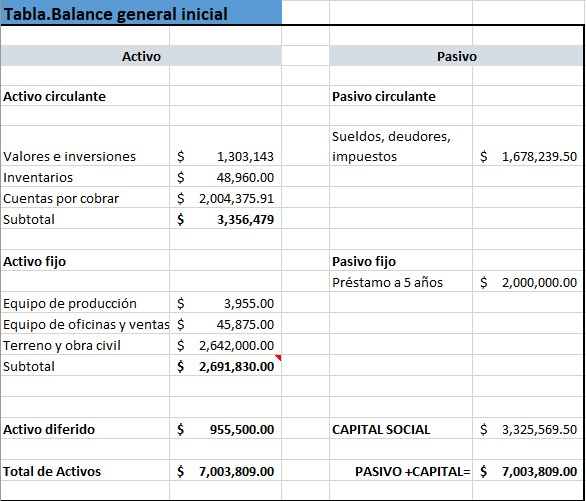
\includegraphics[width=0.9\textwidth]{chapters/ELC_12.png} 
    \caption{Balance general inicial}
\label{fig:croquis190125}
\end{figure}

El balance general inicial mostrará la aportación neta que deberán realizar los accionistas o promotores del proyecto. Notará que la aportación inicial de los accionistas es mucho mayor que los \$45 935 015 calculados para la inversión en activo fijo y diferido, ya que ahora se incluye el capital de trabajo. 

Generalmente para esta aportación adicional se solicita un crédito a corto plazo, recuerde que la naturaleza del capital de trabajo es a corto plazo, no más de tres o cuatro meses; por tanto, los intereses de este préstamo no aparecen en el estado de resultado.




\section{Estado de resultados pro-forma y su evaluación económica con VPN y TIR.}

El estado de resultados pro-forma o proyectado es la base para calcular los flujos netos de efectivo (FNE) con los cuales se realiza la evaluación económica.

Se presentarán tres estados de resultados, las cifras se redondean a miles de pesos; esto es una práctica aceptada cuando
se trabaja con cifras monetarias que se pretende se generen en el futuro.

\subsection{ Estado de resultados sin inflación, sin financiamiento y con producción constante. }

\begin{figure}[H]
    \centering	
    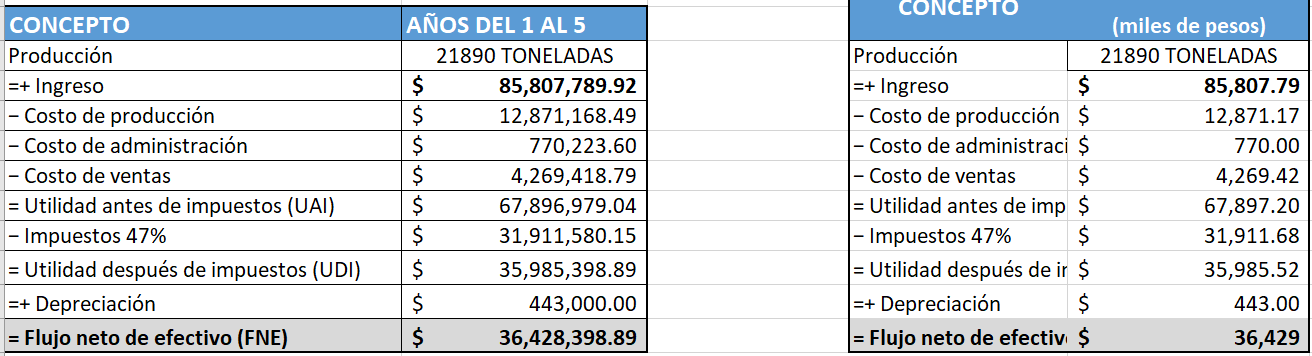
\includegraphics[width=1.1\textwidth]{chapters/ELC_13.png} 
    \caption{Tabla de estado de resultados sin inflación, sin financiamiento y con producción constante}
\label{fig:croquis190125}
\end{figure}

Como la producción es constante y no se toma en cuenta la inflación, entonces la hipótesis es considerar que las cifras de los flujos netos de efectivo se repiten cada fin de año durante todo el horizonte de análisis del proyecto.


\subsection{Estado de resultados con inflación, sin financiamiento y con producción constante.}

\begin{figure}[H]
    \centering	
    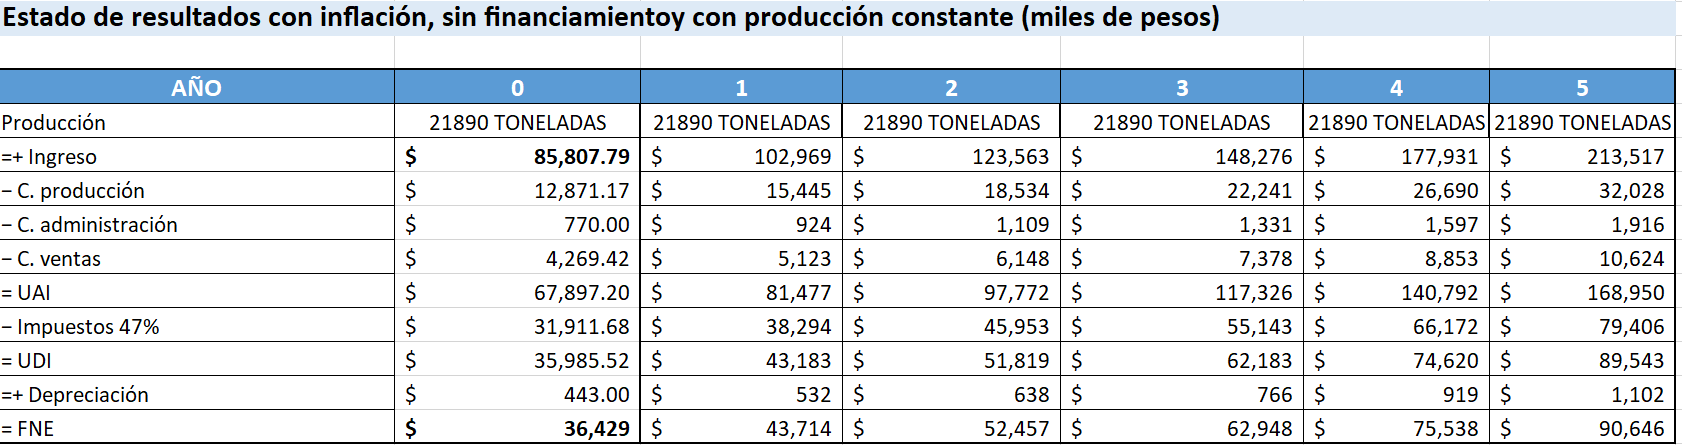
\includegraphics[width=1.1\textwidth]{chapters/ELC_14.png} 
    \caption{Tabla de estado de resultados con inflacón, sin financiamiento y con producción constante}
\label{fig:croquis190125}
\end{figure}

En el plateamiento del estado de resultados, el autor aplica un promedio del aumento de inflación anual de 20\%.  Y considera como el año cero el inicio de la producción para poder aplicar el efecto de la inflación en los años posteriores. Multiplica cada valor del año cero por 1.20.



\subsection{Estado de resultados con inflación, con financiamiento y con producción constante}


\begin{figure}[H]
    \centering	
    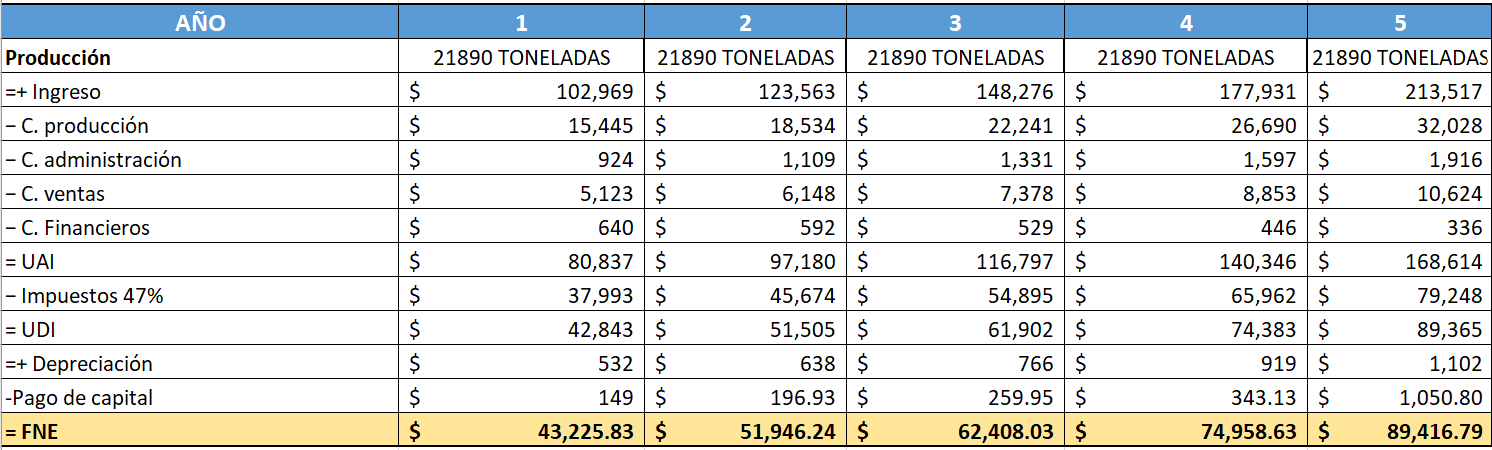
\includegraphics[width=1.1\textwidth]{chapters/ELC_15.png} 
    \caption{Estado de resulatados con inflación, con financiamiento y con roducción constante}
\label{fig:croquis190125}
\end{figure}

 \section{Cálculo del VPN y la TlR con producción variable, sin inflación, con financiamiento}

 \begin{figure}[H]
    \centering	
    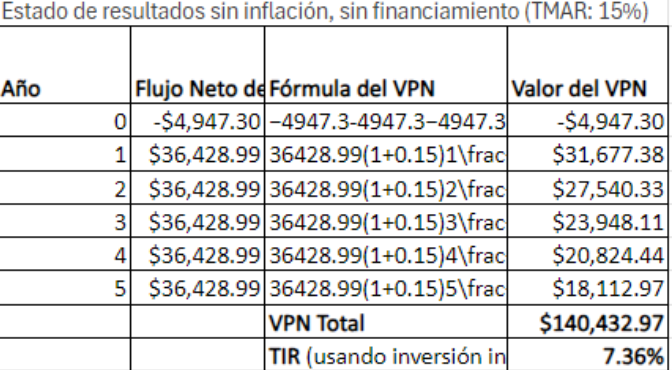
\includegraphics[width=0.7\textwidth]{chapters/ELC_16.png} 
    \caption{Estado de resultados sin inflación,sin financiamiento}
\label{fig:croquis190125}
\end{figure}

\begin{figure}[H]
    \centering	
    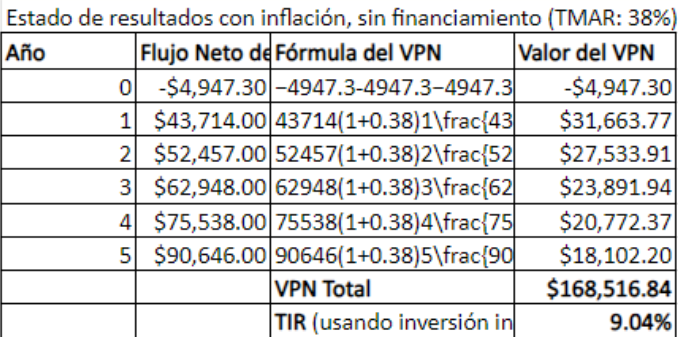
\includegraphics[width=0.7\textwidth]{chapters/ELC_17.png} 
    \caption{Estado de resultados con inflación,sin financiamiento}
\label{fig:croquis190125}
\end{figure}

\begin{figure}[H]
    \centering	
    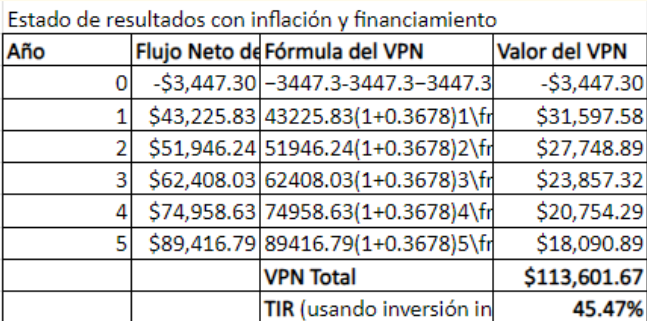
\includegraphics[width=0.7\textwidth]{chapters/ELC_18.png} 
    \caption{Estado de resultados con inflación y financiamiento}
\label{fig:croquis190125}
\end{figure}


\section{Cronograma de inversiones}

Se decidió que el tiempo deseado desde la planeación a la apertura de la empresa sea de 6 meses, por lo que se propone el siguiente calendario. 

\begin{figure}[H]
    \centering	
    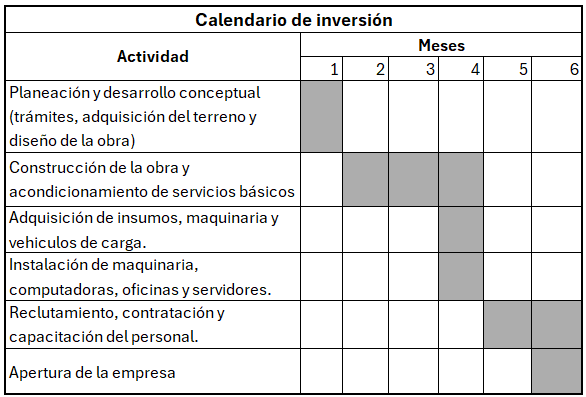
\includegraphics[width=.8\textwidth]{img/Calendario de inversion.png} 
    \caption{Calendario de inversión}
\label{fig:calendarioInversion}
\end{figure}

El calendario está previsto de la siguiente manera sin embargo el reclutamiento y la capacitación del personal se podría adelantar un mes ya que se podrían impartir lecciones teóricas del funcionamiento. 

\section{Conclusiones del estudio económico y evaluación económica}



 El análisis muestra que el proyecto es rentable con un retorno de inversión positivo. Las proyecciones financieras indican que los ingresos generados superarán los costos operativos y de inversión inicial en un plazo razonable.
 Los beneficios derivados de la mejora en la calidad y la cantidad de la producción de flores superan los costos de instalación y operación de las cámaras climáticas.

Se estima que el periodo de recuperación de la inversión inicial es de 5 años, lo cual es aceptable dentro del sector agrícola.
Las proyecciones de ingresos muestran un crecimiento sostenido a lo largo del tiempo, con un aumento en la rentabilidad conforme se estabiliza la operación de las cámaras climáticas.

El análisis detalla los costos iniciales de adquisición e instalación de las cámaras climáticas, así como los gastos en infraestructura y tecnología.

El estudio económico y la evaluación económica del proyecto de cámaras climáticas para flores demuestra que el proyecto es financieramente viable y tiene un potencial significativo para mejorar la producción y calidad de las flores. A través de la implementación de tecnologías avanzadas y prácticas eficientes, el proyecto puede generar beneficios sustanciales tanto para los inversores como para la comunidad local. Además, la capacidad de mitigar riesgos y adaptarse a diferentes escenarios económicos asegura la sostenibilidad a largo plazo del proyecto.